%-----------------------------------------------------------------------------%
\chapter{\babEmpat}
\label{bab:4}
%-----------------------------------------------------------------------------%
Pada Bab Desain dan Implementasi akan dijelaskan mengenai transformasi sistem logistik \f{legacy} menjadi sistem \f{Green Logistics} yang terintegrasi. Pembahasan mencakup gambaran umum arsitektur baru, detail implementasi infrastruktur MLOps untuk prediksi emisi, modifikasi \f{backend} untuk algoritma \f{routing} ramah lingkungan, serta implementasi perangkat keras IoT untuk validasi lapangan.

%-----------------------------------------------------------------------------%
\section{Gambaran Umum Implementasi}
\label{sec:gambaranUmumImplementasi}
%-----------------------------------------------------------------------------%
Implementasi sistem dalam penelitian ini tidak dibangun dari nol, melainkan merupakan evolusi arsitektur dari sistem logistik yang telah dikembangkan pada penelitian sebelumnya (Abdillah et al., 2025). Transformasi sistem dilakukan dengan pendekatan modular, di mana sistem \f{legacy} yang menangani manajemen muatan (\f{Bin Packing Problem}) dipertahankan, sementara modul baru untuk prediksi emisi dan optimasi rute (\f{Green} VRPTW) ditambahkan sebagai layanan terpisah yang terintegrasi.

Untuk memberikan gambaran yang jelas mengenai batasan antara sistem yang sudah ada dan kontribusi baru penelitian ini, arsitektur sistem dijelaskan dalam tiga perspektif visual: Arsitektur \f{Legacy}, Arsitektur Sistem Baru, dan Model Integrasi Antar-Sistem.

%-----------------------------------------------------------------------------%
\subsection{Arsitektur Sistem \f{Legacy}}
\label{sec:arsitekturLegacy}
%-----------------------------------------------------------------------------%
Sistem warisan berfungsi sebagai fondasi operasional logistik. Seperti yang diilustrasikan pada Gambar \ref{fig:arsitekturLegacy}, arsitektur ini berfokus pada pemrosesan data spasial untuk optimasi muatan.

\begin{figure}[t!]
    \centering
    \includegraphics[width=\textwidth]{assets/pics/arsitektur_legacy.png}
    \caption{Arsitektur Sistem \f{Legacy}}
    \label{fig:arsitekturLegacy}
\end{figure}

Komponen utama pada arsitektur ini meliputi:

\begin{enumerate}
    \item \f{Frontend Layer}, terdiri dari Aplikasi iOS untuk pemindaian LiDAR dan \f{Web App} untuk manajemen dasbor.
    
    \item \f{Backend Services}, menggunakan API Gateway (Express.js) sebagai pintu masuk data, PostgreSQL untuk penyimpanan data transaksional, dan RabbitMQ sebagai \f{message broker} untuk mendistribusikan beban kerja. Layanan Django Service di sini berperan sebagai penyedia logika untuk algoritma tata letak boks.
    
    \item \f{GPU Server Cluster}, yaitu sebuah server khusus yang menjalankan kontainer Docker untuk algoritma PointOps (segmentasi dan perhitungan dimensi boks). Komponen ini bekerja secara asinkronus menerima tugas dari RabbitMQ.
\end{enumerate}

%-----------------------------------------------------------------------------%
\subsection{Arsitektur Sistem \f{Green Logistics} (\f{New System})}
\label{sec:arsitekturGreenLogistics}
%-----------------------------------------------------------------------------%
Untuk mendukung fitur \f{Green} VRPTW, penelitian ini membangun infrastruktur baru yang disebut sebagai \f{Green Engine}. Infrastruktur ini dirancang dengan prinsip \f{Machine Learning Operations} (MLOps) untuk menangani komputasi emisi yang intensif. Detail arsitektur baru ini ditampilkan pada Gambar \ref{fig:arsitekturNewSystem}.

\begin{figure}[t!]
    \centering
    \includegraphics[width=\textwidth]{assets/pics/arsitektur_new_system.png}
    \caption{Arsitektur Infrastruktur MLOps dan IoT (\f{New System})}
    \label{fig:arsitekturNewSystem}
\end{figure}

Komponen baru yang dikembangkan meliputi:

\begin{itemize}
    \item \f{MLOps Infrastructure} \\
    Menggunakan Apache Airflow sebagai orkestrator utama yang mengatur eksekusi \f{worker} untuk model Markov Chain (MCM) dan model emisi MOVESTAR. Seluruh data tidak terstruktur (\f{model artifact} dan hasil prediksi) disimpan dalam MinIO, sebuah \f{Object Storage} yang kompatibel dengan protokol S3.
    
    \item \f{IoT Validation Hardware} \\
    Perangkat keras berbasis mikrokontroler Arduino Uno R4 yang dilengkapi sensor gas (\ce{CO2}, CO, HC). Perangkat ini bekerja secara independen untuk merekam data emisi riil ke kartu SD, yang kemudian diunggah secara \f{batch} ke MinIO untuk keperluan validasi model.
\end{itemize}

%-----------------------------------------------------------------------------%
\subsection{Integrasi dan Alur Komunikasi Sistem}
\label{sec:integrasiAlurKomunikasi}
%-----------------------------------------------------------------------------%
Tantangan utama dalam implementasi ini adalah menghubungkan logika bisnis pada \f{legacy backend} (Django) dengan kemampuan komputasi pada \f{Green Engine} (Airflow). Integrasi dilakukan menggunakan pola komunikasi asinkronus berbasis API, sebagaimana digambarkan pada Gambar \ref{fig:modelIntegrasi}.

\begin{figure}
    \centering
    \includegraphics[width=0.6\textwidth]{assets/pics/model_integrasi.png}
    \caption{Model Integrasi \f{Legacy Backend} dan \f{Green Engine}}
    \label{fig:modelIntegrasi}
\end{figure}

Alur komunikasi antar-sistem berjalan sebagai berikut:

\begin{enumerate}
    \item \f{Trigger Inference} \\
    Saat pengguna meminta rekomendasi rute hijau, layanan Django mengirimkan permintaan HTTP POST ke REST API Airflow untuk memicu \f{pipeline} inferensi.
    
    \item Proses Komputasi \\
    Airflow menjalankan DAGs yang menghitung prediksi emisi dan menyimpan hasilnya dalam format JSON ke dalam \f{Data Lake} (MinIO).
    
    \item \f{Polling} \& \f{Fetch} \\
    Karena proses prediksi membutuhkan waktu, Django melakukan mekanisme \f{polling} (pengecekan berkala) terhadap status tugas di Airflow. Setelah status dinyatakan sukses, Django mengambil (\f{fetch}) data hasil emisi dari MinIO untuk dikonversi menjadi matriks biaya (\f{cost matrix}) dalam penentuan rute.
\end{enumerate}

%-----------------------------------------------------------------------------%
\section{Implementasi MLOps dan Model Emisi}
\label{sec:implementasiMLOps}
%-----------------------------------------------------------------------------%
Bagian ini membahas implementasi teknis dari "mesin" prediksi emisi yang menjadi inti dari \f{Green} VRPTW. Implementasi ini mencakup infrastruktur orkestrasi, model pembangkit siklus berkendara, dan model perhitungan emisi.

Secara konseptual, alur kerja sistem rekomendasi rute ini tidak hanya melibatkan perhitungan jarak, tetapi juga integrasi data topologi dan prediksi. Ilustrasi cara kerja sistem dari \f{input} pengguna hingga visualisasi hasil dapat dilihat pada Gambar \ref{fig:greenRoutingWorkflow}.

\begin{figure}[ht]
    \centering
    \includegraphics[width=0.3\textwidth]{assets/pics/green_routing_workflow.png}
    \caption{Alur Kerja Sistem Rekomendasi Rute (\f{Green Routing Workflow})}
    \label{fig:greenRoutingWorkflow}
\end{figure}

%-----------------------------------------------------------------------------%
\subsection{Infrastruktur Airflow \& MinIO}
\label{sec:infrastrukturAirflowMinIO}
%-----------------------------------------------------------------------------%
Untuk menangani kompleksitas orkestrasi model yang melibatkan berbagai tahapan sekuensial, digunakan Apache Airflow sebagai \f{workflow engine}. Implementasi ini membagi proses komputasi menjadi beberapa \f{Directed Acyclic Graphs} (DAGs) terpisah guna menjaga modularitas sistem. Berikut adalah detail implementasi dua \f{pipeline} utama yang divisualisasikan melalui \f{Graph View} pada antarmuka Airflow.

\begin{enumerate}
    \item \f{Pipeline Ingest Data} (\code{01\_ingest\_new\_zips})
    
    \f{Pipeline} ini bertanggung jawab atas pemrosesan awal data mentah (\f{raw data}) yang dikirimkan oleh Sensor Logger. Seperti yang ditunjukkan pada Gambar \ref{fig:pipelineIngestGraph}, struktur DAG ini didesain menggunakan pola \f{Dynamic Task Mapping}.
    
    \begin{figure}
        \centering
        \includegraphics[width=\textwidth]{assets/pics/pipeline_ingest_graph.png}
        \caption{Visualisasi \f{Graph View} untuk \f{Pipeline Ingest} pada Apache Airflow}
        \label{fig:pipelineIngestGraph}
    \end{figure}
    
    Alur eksekusi pada DAG ini terdiri dari dua \f{task} utama:
    \begin{itemize}
        \item \code{get\_new\_trips} \\
        Sebuah \f{Python Operator} yang memindai \f{bucket} S3 \code{raw-gps} untuk mendeteksi berkas ZIP baru yang belum diproses. \f{Task} ini menghasilkan daftar ID perjalanan (\f{list of trip IDs}) yang diteruskan ke \f{task} berikutnya.
        \item \code{process\_trip} \\
        Sebuah \f{Papermill Operator} yang dipetakan secara dinamis (\f{mapped task}) untuk setiap ID perjalanan yang ditemukan. \f{Task} ini mengeksekusi Jupyter Notebook \code{00\_ingest\_raw\_trip.ipynb} secara paralel. Di dalam \f{notebook} ini, terjadi proses \f{sensor fusion} (penggabungan data akselerometer dan GPS), \f{resampling} data ke frekuensi 1 Hz, dan penyelarasan rute (\f{map matching}), sebelum akhirnya menyimpan data bersih ke \f{bucket} \code{processed-data}.
    \end{itemize}

    \item \f{Pipeline} Inferensi (\code{03\_inference\_pipeline})
    
    \f{Pipeline} ini adalah inti dari sistem \f{Green Routing}, yang dijalankan secara \f{on-demand} ketika ada permintaan dari \f{backend}. Gambar \ref{fig:pipelineInferenceGraph} memperlihatkan struktur linear dari \f{pipeline} ini, yang menjamin urutan eksekusi logis dari pengambilan data spasial hingga perhitungan emisi.
    
    \begin{figure}
        \centering
        \includegraphics[width=\textwidth]{assets/pics/pipeline_inference_graph.png}
        \caption{Visualisasi \f{Graph View} untuk \f{Pipeline Inference} pada Apache Airflow}
        \label{fig:pipelineInferenceGraph}
    \end{figure}
    
    Setiap \f{node} dalam grafik merepresentasikan langkah komputasi spesifik:
    \begin{itemize}
        \item \code{step\_04\_fetch\_topology} \\
        Langkah ini memegang peranan vital karena Google Maps Platform digunakan sebagai penyedia data konteks lingkungan (\f{Environmental Context Provider}), bukan sekadar peta visual. \f{Task} ini mengekstraksi fitur topologi jalan yang menjadi bahan utama model ML, meliputi:
        \begin{enumerate}
            \item \textbf{Koordinat Geometri (\f{Polyline}):} Digunakan untuk mendeteksi pola belokan tajam yang memungkinkan model memprediksi momen deselerasi.
            \item \textbf{Data Elevasi (\f{Elevation Gain}):} Sistem mengambil profil ketinggian untuk menghitung gradien kemiringan jalan (tanjakan/turunan).
        \end{enumerate}
        
        \item \code{step\_05\_generate\_cycle} \\
        Menggunakan model Markov Chain (atau ML) yang telah dilatih untuk membangkitkan profil kecepatan sintetis (\f{drive cycle}) yang sesuai dengan karakteristik topologi rute (tanjakan dan belokan) yang didapat dari tahap sebelumnya.
        
        \item \code{step\_06\_movestar} \\
        Mengambil profil kecepatan sebagai \f{input} untuk menghitung estimasi emisi total menggunakan model MOVESTAR. Hasil akhirnya disimpan sebagai objek JSON di MinIO agar dapat diambil oleh layanan Django.
    \end{itemize}
    
    Penggunaan Airflow memungkinkan pemantauan visual terhadap status setiap langkah (\f{success/failed}) dan menyediakan mekanisme \f{retry} otomatis jika terjadi kegagalan pada salah satu \f{node}, meningkatkan reliabilitas sistem secara keseluruhan.
\end{enumerate}

%-----------------------------------------------------------------------------%
\subsection{Implementasi Markov Chain (MCM)}
\label{sec:implementasiMarkovChain}
%-----------------------------------------------------------------------------%
Inti dari pembangkitan siklus berkendara sintetis adalah model Markov Chain yang memetakan dinamika pergerakan kendaraan ke dalam ruang keadaan diskrit. Implementasi dimulai dengan pendefinisian Ruang Keadaan (\f{State Space}) dalam bentuk \f{grid} 2D yang merepresentasikan pasangan nilai kecepatan ($v$) dan akselerasi ($a$).

Dalam penelitian ini, data perjalanan dikelompokkan menjadi dua segmen utama berdasarkan karakteristik lalu lintas: \f{Heavy Traffic} (Lalu Lintas Padat) dan \f{Light Traffic} (Lalu Lintas Lancar). Pengelompokan ini penting karena perilaku berkendara dan pola emisi yang dihasilkan bisa sangat berbeda pada kedua kondisi tersebut.

Pengelompokan data \f{training} dilakukan berdasarkan kecepatan rata-rata segmen perjalanan. Segmen dengan kecepatan rata-rata di bawah 25 km/jam dikategorikan sebagai \f{Heavy Traffic}, sedangkan segmen dengan kecepatan di atas atau sama dengan 25 km/jam dikategorikan sebagai \f{Light Traffic}.

%-----------------------------------------------------------------------------%
\subsubsection{Visualisasi Grid Keadaan}
\label{sec:visualisasiGridKeadaan}
%-----------------------------------------------------------------------------%
Proses diskretisasi data divisualisasikan dalam bentuk \f{Speed-Acceleration Grid Map}. Setiap titik biru pada peta merepresentasikan satu detik data perjalanan ($v_t, a_t$), sedangkan angka merah menunjukkan ID \f{State} unik yang diberikan pada setiap sel \f{grid}.

\begin{figure}[t!]
    \centering
    \includegraphics[width=\textwidth]{assets/pics/grid_map_heavy_traffic.png}
    \caption{Peta \f{Grid} Kecepatan-Akselerasi untuk Kondisi \f{Heavy Traffic} (SEG0)}
    \label{fig:gridMapHeavy}
\end{figure}

Gambar \ref{fig:gridMapHeavy} menunjukkan distribusi \f{state} pada kondisi lalu lintas padat (\f{Heavy Traffic}). Terlihat konsentrasi titik data yang sangat tinggi pada area kecepatan rendah (0 - 20 km/jam) dengan variasi akselerasi yang rapat. Hal ini mencerminkan karakteristik \f{stop-and-go} di mana kendaraan sering berhenti, berakselerasi pendek, dan mengerem kembali. Jumlah \f{state} yang teridentifikasi (mencapai \f{state} ke-185) menunjukkan kompleksitas manuver pada kondisi macet.

\begin{figure}[t!]
    \centering
    \includegraphics[width=\textwidth]{assets/pics/grid_map_light_traffic.png}
    \caption{Peta \f{Grid} Kecepatan-Akselerasi untuk Kondisi \f{Light Traffic} (SEG1)}
    \label{fig:gridMapLight}
\end{figure}

Sebaliknya, Gambar \ref{fig:gridMapLight} memperlihatkan distribusi untuk kondisi lalu lintas lancar (\f{Light Traffic}). Persebaran titik data lebih merata ke arah kanan sumbu kecepatan ($> 30$ km/jam), mengindikasikan kendaraan dapat melaju lebih cepat dan stabil. Jumlah \f{state} yang lebih sedikit (sampai \f{state} ke-90) menunjukkan pola berkendara yang lebih konsisten dan minim fluktuasi ekstrem dibandingkan saat macet.

%-----------------------------------------------------------------------------%
\subsubsection{Pembangkitan Matriks Transisi}
\label{sec:pembangkitanMatriksTransisi}
%-----------------------------------------------------------------------------%
Berdasarkan pemetaan \f{state} pada kedua gambar di atas, kode program menghitung matriks probabilitas transisi secara terpisah untuk setiap segmen. Matriks ini menyimpan peluang perpindahan dari satu ID \f{state} ke ID \f{state} lainnya (misalnya, peluang berpindah dari \f{State} 10 ke \f{State} 11). Fungsi \code{generate\_cycle} kemudian menggunakan matriks yang relevan---apakah matriks \f{Heavy} atau \f{Light}---bergantung pada prediksi kondisi lalu lintas dari Google Maps untuk membangkitkan profil kecepatan sintetis yang akurat.

%-----------------------------------------------------------------------------%
%-----------------------------------------------------------------------------%
\section{Implementasi Model \f{Machine Learning} (ML)}
\label{sec:implementasiML}
%-----------------------------------------------------------------------------%
Berbeda dengan pendekatan Markov Chain yang memodelkan probabilitas transisi antar-\f{state}, pendekatan \f{machine learning} (ML) dalam penelitian ini memandang permasalahan prediksi \f{drive cycle} sebagai masalah regresi \f{time-series}. Tujuannya adalah melatih model komputasi untuk memprediksi kecepatan kendaraan pada detik berikutnya ($v_{t+1}$, $a_{t+1}$) berdasarkan serangkaian fitur historis dan kontekstual pada detik sebelumnya. Seluruh rangkaian eksperimen ini ada di dalam \f{orchestrator} Apache Airflow untuk menjamin reproduksibilitas proses, mulai dari pembagian data, pelatihan model, hingga validasi kualitas model.

%-----------------------------------------------------------------------------%
\subsection{Pengambilan \f{Dataset}}
\label{sec:pengambilanDataset}
%-----------------------------------------------------------------------------%
\f{Dataset} yang digunakan dalam penelitian ini bersumber dari rekaman perjalanan kendaraan secara riil di lapangan menggunakan perangkat sensor yang telah dikalibrasi. Proses akuisisi data dilakukan selama total 8 jam waktu operasional, yang mencakup berbagai kondisi lalu lintas dan karakteristik jalan. Untuk menjamin kualitas model dalam melakukan generalisasi pada rute yang berbeda, \f{dataset} dibagi menjadi dua kategori utama dengan skenario lokasi sebagai berikut:

\begin{enumerate}
    \item Dataset Pelatihan (\f{Training Set}) \\
    Data diambil dari rute perjalanan Pamulang (Tangerang Selatan) menuju Universitas Indonesia (Depok) dan sebaliknya dengan estimasi jarak tempuh berada di kisaran 25-30 KM untuk sekali perjalanan. Rute ini dipilih untuk memberikan representasi pola berkendara yang bervariasi, mulai dari jalan arteri dengan kecepatan tinggi hingga kondisi lalu lintas padat di area penghubung antar kota. Seluruh kombinasi rute yang diambil memiliki titik awal dan titik akhir yang sama dengan varian rute yang berbeda. Selama tahap pengambilan data untuk keperluan dataset pelatihan ini, masing-masing rute dapat dilewati lebih dari satu kali. Adapun rute-rute diambil dari kombinasi sebagai berikut.
    
    \begin{figure}[t!]
        \centering
        \includegraphics[width=\textwidth]{assets/pics/kombinasi_pp.png}
        \caption{Visualisasi Kombinasi Rute Dataset Pelatihan Menggunakan Google Maps}
        \label{fig:kombinasiPP}
    \end{figure}

    \item Dataset Pengujian (\f{Testing Set}) \\
    Data diambil dari rute perjalanan keliling di wilayah sekitar Universitas Indonesia hingga area Kukusan. Pemilihan rute pengujian di lokasi yang berbeda dari data pelatihan bertujuan untuk mengevaluasi kemampuan model dalam menggeneralisasi pola \f{drive cycle} pada segmen jalan lingkungan dan perkotaan yang didominasi oleh perilaku \f{stop-and-go}. Seluruh kombinasi rute yang diambil memiliki titik awal dan titik akhir yang sama dengan varian rute yang berbeda. Adapun rute-rute diambil dari kombinasi sebagai berikut.
    
    \begin{figure}
        \centering
        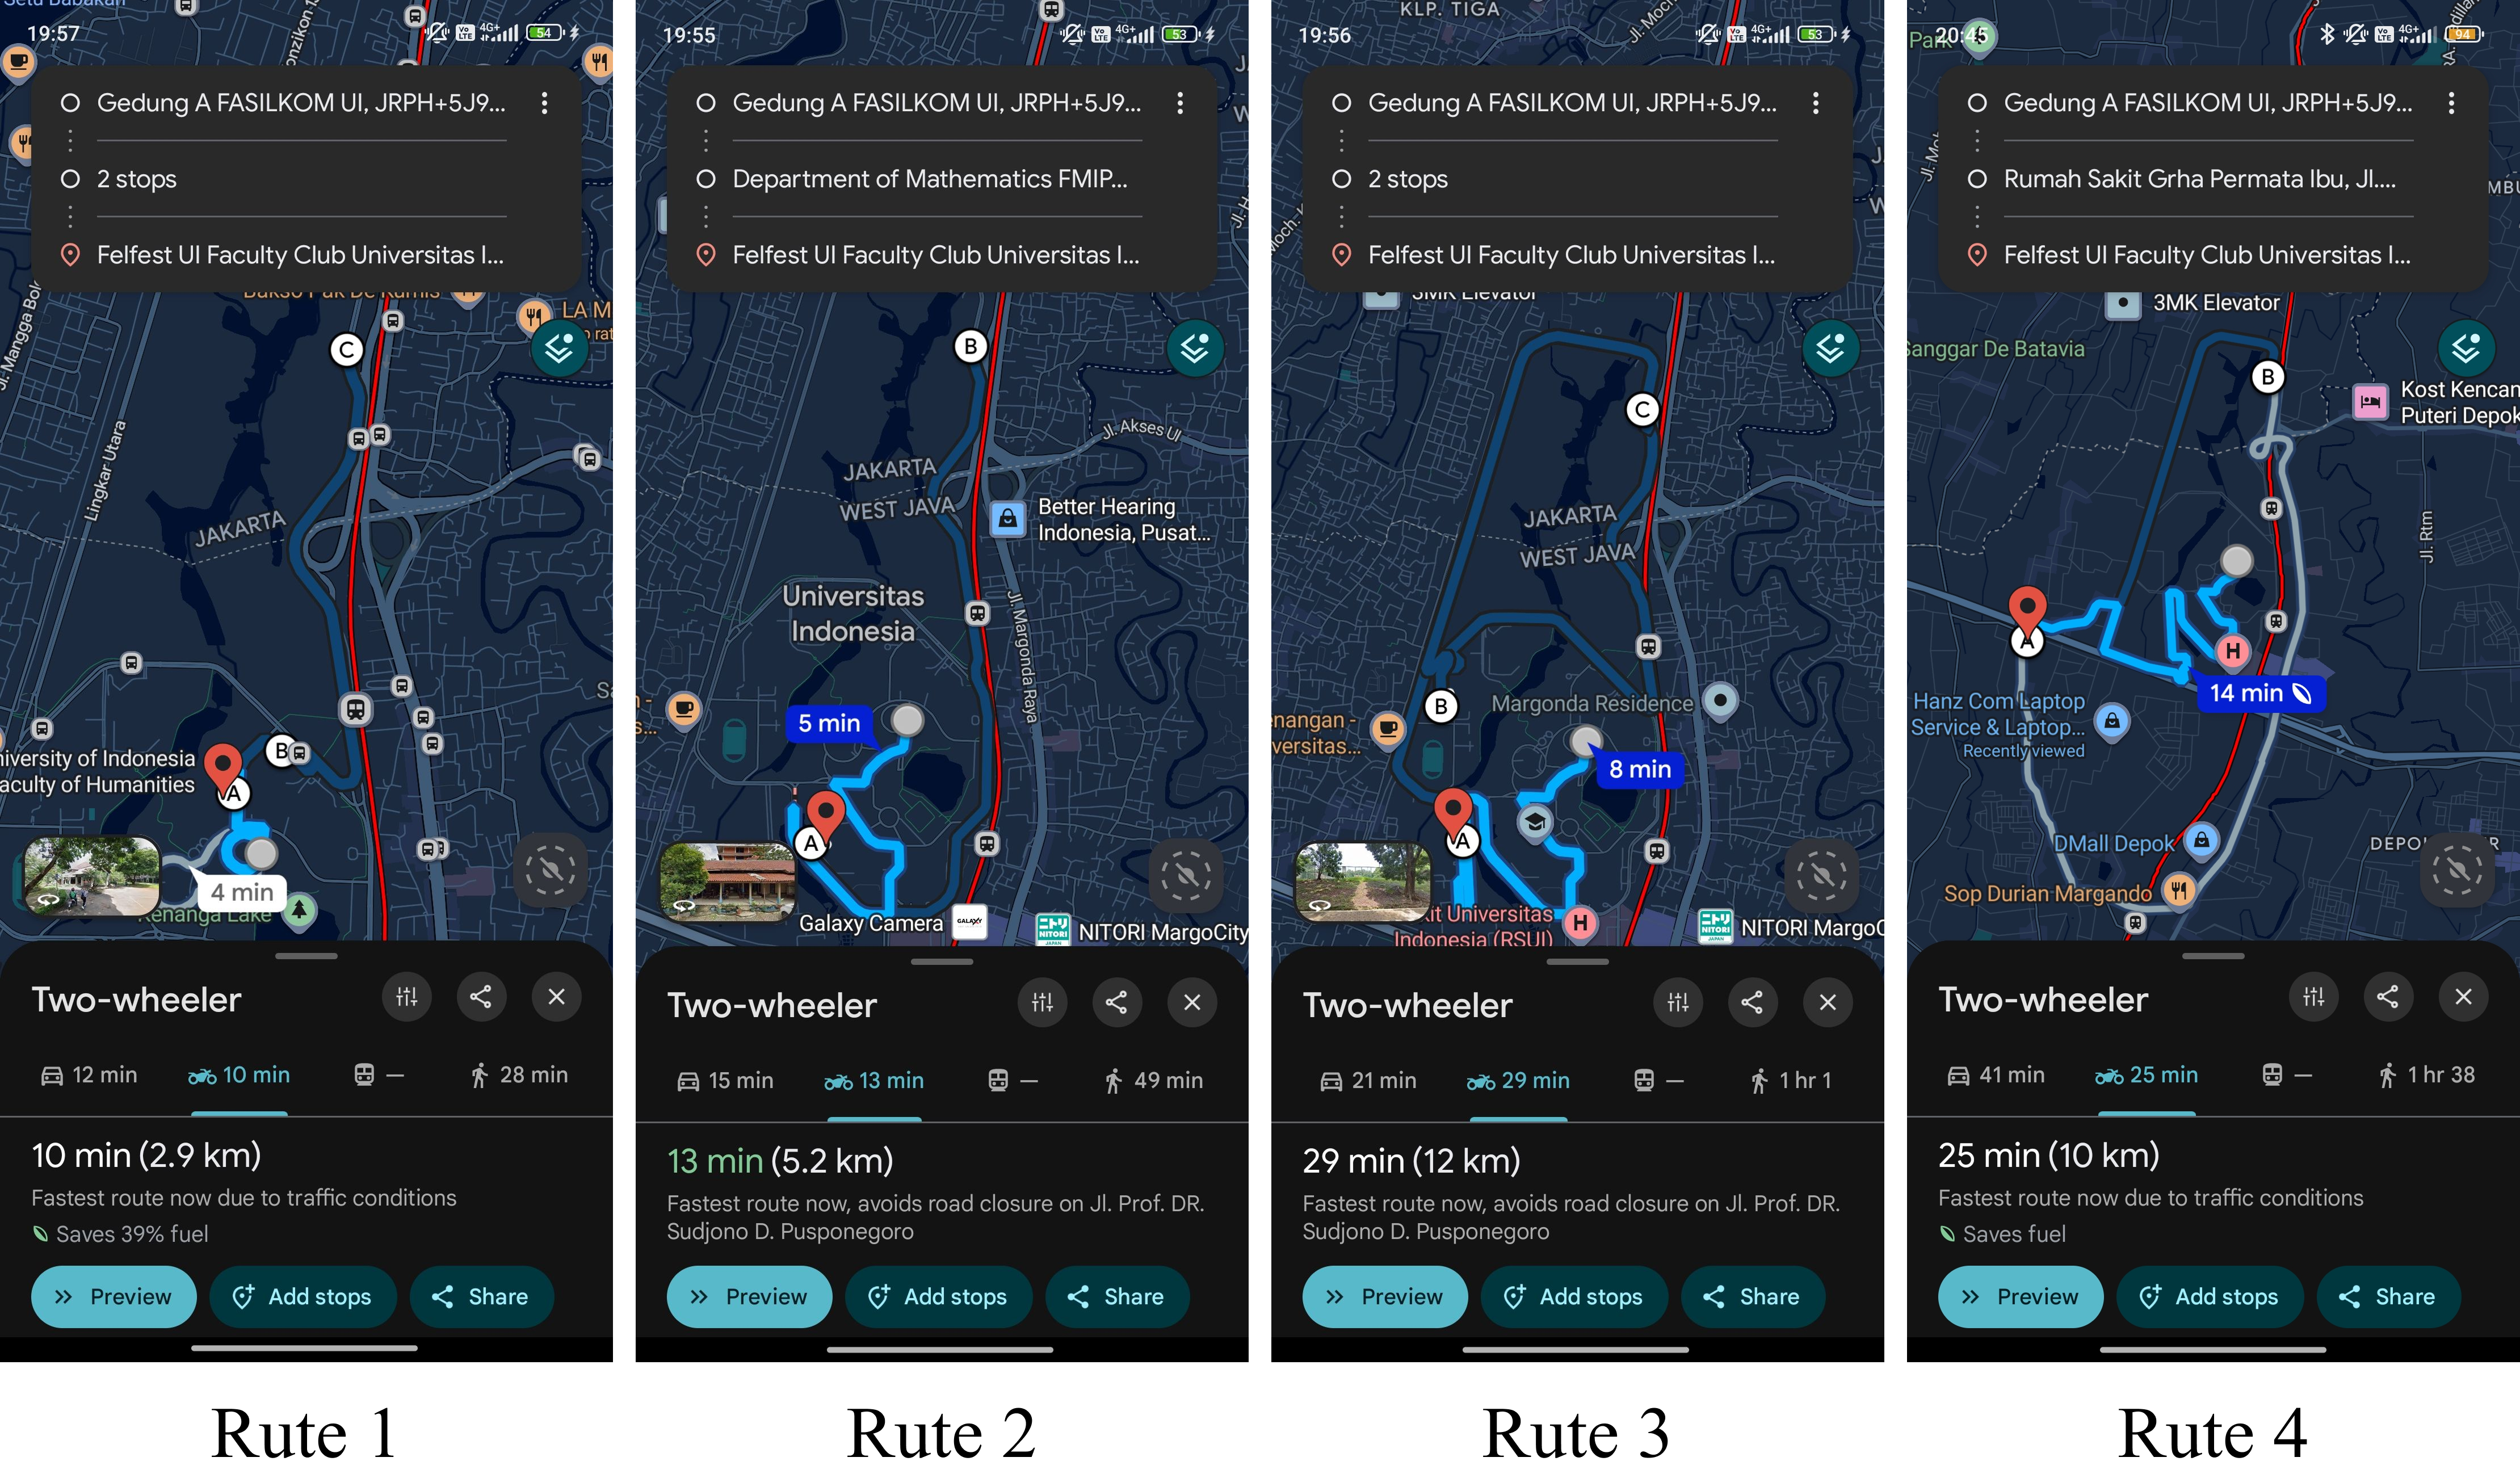
\includegraphics[width=\textwidth]{assets/pics/kombinasi_testing_ui.png}
        \caption{Visualisasi Kombinasi Rute Dataset Pengujian Menggunakan Google Maps}
        \label{fig:kombinasiRuteUI}
    \end{figure}
\end{enumerate}

Sistem melakukan penggabungan beberapa rekaman perjalanan yang telah terkumpul di dalam penyimpanan awan (\f{cloud storage}) MinIO menjadi satu kesatuan \f{dataset} yang utuh. Berdasarkan proses tersebut, diperoleh distribusi data sebagai berikut:

\begin{figure}[t!]
    \centering
    \includegraphics[width=0.7\textwidth]{assets/pics/dataset_split_log.png}
    \caption{\f{Log} Pembagian \f{Dataset} Pelatihan dan Pengujian}
    \label{fig:datasetSplit}
\end{figure}

\begin{itemize}
    \item Data Pelatihan: Terdiri dari penggabungan 9 rekaman perjalanan utama (seperti rekaman rute jalan arteri dan jalan penghubung) dengan total volume sebanyak 24.026 titik data (detik).
    \item Data Pengujian: Terdiri dari penggabungan 3 rekaman perjalanan independen di area lingkungan sekitar kampus dengan total volume sebanyak 5.006 titik data (detik).
\end{itemize}

Pembagian ini menghasilkan rasio yang ideal untuk fase pembelajaran model dalam menangkap kompleksitas hubungan antara fitur \f{input} dan profil kecepatan kendaraan secara mendalam. Meskipun secara kuantitas volume data dalam penelitian ini lebih kecil dibandingkan referensi utama \citep{de2021microscopic} sejumlah 29.032 titik data (detik), integritas data dijaga melalui proses \f{sampling} 1 Hz yang sinkron antara data GPS dan sensor inersia.

Selain itu, data operasional dikumpulkan secara mandiri pada rute yang terkontrol (BSD–UI dan UI–Kukusan), sehingga setiap titik data memiliki konteks lingkungan yang konsisten. Kondisi ini memungkinkan model mempelajari keterkaitan antara karakteristik geometri jalan dan dinamika kendaraan dengan lebih fokus. Selain itu, digunakan satu tipe kendaraan, sehingga menghindari gangguan variasi tipe kendaraan yang umumnya terdapat pada \f{dataset} publik berskala besar.

%-----------------------------------------------------------------------------%
\subsection{Persiapan Data dan \f{Feature Engineering}}
\label{sec:featureEngineeringImpl}
%-----------------------------------------------------------------------------%
Kualitas prediksi model \f{machine learning} tentu bergantung pada kualitas fitur \f{input} yang digunakan. Sebagaimana telah dibahas pada Subbab 3.4.3, pemilihan variabel dalam penelitian ini bertujuan untuk mentransformasikan informasi jalan statis (makroskopik) menjadi estimasi dinamika pergerakan (mikroskopik).

%-----------------------------------------------------------------------------%
\subsubsection{Implementasi \f{Derived Acceleration} (Akselerasi Turunan)}
\label{sec:derivedAccelerationImpl}
%-----------------------------------------------------------------------------%
Berdasarkan hasil observasi pada data sensor mentah, ditemukan bahwa variabel akselerasi langsung dari alat (\code{acc\_forward}) memiliki tingkat \f{noise} yang sangat tinggi dan fluktuasi yang tidak konsisten akibat guncangan kendaraan. Untuk mengatasi hal ini, diterapkan strategi \f{derived acceleration}. Akselerasi tidak diambil dari sensor, melainkan dihitung secara matematis sebagai turunan pertama dari kecepatan terhadap waktu:

\begin{equation}
    a = \frac{v_t - v_{t-1}}{\Delta t}
\end{equation}

Di mana $\Delta t = 1$ detik (sesuai frekuensi \f{sampling}). Pendekatan ini menjamin konsistensi fisik antara profil kecepatan dan akselerasi, yang sangat krusial saat nilai tersebut digunakan untuk menghitung emisi pada model MOVESTAR.

%-----------------------------------------------------------------------------%
\subsubsection{Kategorisasi Fitur \f{Input}}
\label{sec:kategorisasiFitur}
%-----------------------------------------------------------------------------%
Fitur-fitur yang diekstraksi dalam penelitian ini dirancang untuk memberikan pemahaman konteks yang multidimensi bagi model \f{machine learning}. Seluruh variabel \f{input} (total 18 fitur) dikelompokkan ke dalam empat kategori utama guna menangkap aspek fisik kendaraan, tren pergerakan, geometri jalan, dan kondisi lalu lintas secara implisit:

\begin{enumerate}[label=\alph*)]
    \item Dinamika Kendaraan dan Autoregresif (\f{Autoregressive Dynamics}) \\
    Kategori ini menangkap kondisi fisik sesaat dan inersia kendaraan. Variabel yang digunakan adalah: \code{speed\_mps\_prev1}, \code{speed\_mps\_prev2}, dan \code{accel\_prev1}. Mengikuti prinsip rantai Markov dan ketergantungan temporal, fitur ini memastikan prediksi kecepatan detik berikutnya bersifat berkelanjutan (\f{continuous}). Dengan menyertakan kecepatan dan akselerasi dari dua langkah waktu sebelumnya, model dapat memahami tren percepatan atau perlambatan yang sedang terjadi, sehingga mencegah perubahan kecepatan yang tidak logis secara fisik.

    \item Statistik Tren dan Momentum (\f{Rolling Statistics \& Momentum}) \\
    Kategori ini memberikan konteks mengenai stabilitas pergerakan dalam jendela waktu 5 detik. Rata-rata bergerak atau \f{rolling mean} (\code{speed\_roll\_mean\_5s}) memberikan gambaran momentum kendaraan selama 5 detik. Sementara itu, standar deviasi bergerak atau \f{rolling std} (\code{speed\_roll\_std\_5s}) berfungsi sebagai indikator volatilitas. Nilai deviasi yang tinggi mengindikasikan perilaku berkendara yang agresif atau kondisi \f{stop-and-go}, yang sangat mempengaruhi lonjakan emisi pada model MOVESTAR.

    \item Konteks Spasial dan Geometri Jalan (\f{Spatial \& Geometric Context}) \\
    Kategori ini memetakan pengaruh lingkungan fisik dan topografi rute terhadap beban mesin. \code{delta\_dist} merupakan fitur yang menjelaskan perpindahan posisi, yang didapat dari jarak \f{euclidian} dari posisi \f{longitude} dan \f{latitude}. Perubahan elevasi (\code{elev\_gain\_m}) secara langsung mempengaruhi nilai \f{Grade} dalam perhitungan VSP. Sementara itu, fitur geometri seperti perubahan arah (\code{heading\_change}) dan jumlah belokan (\code{turn\_count}) memberikan sinyal kepada model bahwa kendaraan kemungkinan besar akan melambat saat menghadapi tikungan atau persimpangan, terlepas dari kondisi lalu lintas.

    \item Karakteristik Segmen dan Batas Jalan (\f{Road Segment Characteristics}) \\
    Kategori ini menetapkan "koridor" atau batas atas perilaku berkendara pada segmen tertentu. \code{segment\_avg\_speed} merupakan nilai rata-rata kecepatan dalam satu segmen jalan (yang diambil dari Google Maps API) yang cukup krusial pada saat inferensi. \code{speed\_limit\_kmh} berfungsi sebagai referensi statis aturan jalan. \code{speed\_ratio} (rasio antara kecepatan saat ini dengan batas kecepatan) menjadi fitur kunci yang memungkinkan model untuk generalisasi perilaku pada rute baru. Jika rasio rendah secara konsisten, model mempelajari bahwa segmen tersebut memiliki hambatan tinggi.

    \item Indikator Lalu Lintas Implisit dan Peristiwa Berhenti (\f{Implicit Traffic \& Events}) \\
    Kategori ini adalah hasil rekayasa fitur cerdas untuk menggantikan peran data \f{real-time} eksternal. \code{speed\_drop} berfungsi untuk mengidentifikasi besarnya penurunan kecepatan secara signifikan antar detik guna menandai fase perlambatan. Selanjutnya, \code{traffic\_shock} berperan mendeteksi anomali perlambatan mendadak yang menjadi indikator adanya kepadatan kendaraan atau gangguan aliran lalu lintas di depan rute. Untuk mendeteksi status operasional kendaraan secara langsung, \code{stop\_flag} digunakan sebagai penanda biner (0 atau 1) yang mengidentifikasi apakah kendaraan sedang berada dalam kondisi berhenti total atau diam di tempat. Terakhir, \code{stop\_density\_20s} bekerja dengan menghitung frekuensi atau seberapa sering kendaraan berhenti dalam durasi singkat (jendela waktu 20 detik), yang secara implisit memetakan tingkat kemacetan rute atau keberadaan infrastruktur jalan seperti lampu lalu lintas tanpa memerlukan koneksi ke API pihak ketiga.
\end{enumerate}

%-----------------------------------------------------------------------------%
\subsubsection{Konsistensi Struktur Fitur Pelatihan dan Inferensi}
\label{sec:konsistensiFitur}
%-----------------------------------------------------------------------------%
Aspek krusial dalam implementasi ini adalah penggunaan variabel \code{speed\_ratio} dan \code{speed\_limit\_kmh} untuk menjamin konsistensi struktur \f{input} model. Pada tahap pelatihan, kedua variabel ini diinisialisasi dengan nilai konstan untuk memenuhi prinsip keseragaman fitur antara tahap pelatihan dan inferensi sebagaimana dijabarkan pada Subbab 3.4.3. Peran fungsional kedua variabel ini menjadi sangat vital pada tahap inferensi, mengingat model tidak memiliki akses ke data kecepatan dasar (\f{ground truth speed}) pada rute baru. Maka dari itu, \code{speed\_limit\_kmh} dan \code{speed\_ratio} berperan sebagai batas koridor fisik (\f{boundary conditions}) untuk memandu model dalam menghasilkan profil kecepatan sintetis yang realistis dan patuh terhadap regulasi jalan yang berlaku.

%-----------------------------------------------------------------------------%
\subsection{Pelatihan dan Seleksi Model}
\label{sec:pelatihanSeleksi}
%-----------------------------------------------------------------------------%
Proses pelatihan model merupakan tahap di mana algoritma mempelajari korelasi antara fitur kontekstual jalan dengan dinamika kecepatan kendaraan secara mikroskopik. Tahap ini dieksekusi melalui tugas \code{step\_05\_generate\_cycle} pada \f{pipeline} Airflow menggunakan \f{dataset} pelatihan (\code{train\_data.pkl}) yang mencakup 80\% dari total populasi \f{dataset}.

%-----------------------------------------------------------------------------%
\subsubsection{Pra-pemrosesan dan Standardisasi}
\label{sec:prapemrosesan}
%-----------------------------------------------------------------------------%
Sebelum proses pelatihan dimulai, fitur \f{input} melalui tahap standarisasi menggunakan StandardScaler. Langkah ini krusial untuk memastikan setiap fitur memiliki rata-rata nol dan standar deviasi satu, sehingga algoritma yang sensitif terhadap skala data dapat mencapai konvergensi yang optimal. Hal ini terutama berlaku bagi model \f{Support Vector Regression} (SVR) dan \f{Artificial Neural Networks} (ANN), sebagaimana dijelaskan pada Subbab 2.3.3.1, di mana skala data yang seragam membantu fungsi kernel dan mekanisme \f{backpropagation} bekerja lebih efektif.

%-----------------------------------------------------------------------------%
\subsubsection{Implementasi Algoritma Pembanding}
\label{sec:implementasiAlgoritma}
%-----------------------------------------------------------------------------%
Penelitian ini membandingkan lima algoritma regresi non-linear untuk menemukan model yang paling presisi dalam menangkap variabilitas \f{drive cycle}. Pemilihan algoritma ini didasarkan pada tinjauan literatur yang mendalam pada Bab 2 dan Bab 3.

\begin{itemize}
    \item \f{Artificial Neural Networks} (ANN)
    \item XGBoost
    \item \f{Random Forest} (RF)
    \item \f{Support Vector Regression} (SVR)
    \item \f{Decision Tree} (DT)
\end{itemize}

%-----------------------------------------------------------------------------%
\subsubsection{Konfigurasi \f{Hyperparameter} dan Validasi}
\label{sec:konfigurasiHyperparameter}
%-----------------------------------------------------------------------------%
Penentuan parameter optimal untuk setiap algoritma dilakukan melalui tahap eksperimen awal (\f{pre-tuning}) untuk menyeimbangkan akurasi dan risiko \f{overfitting}. Beberapa konfigurasi utama meliputi:

\begin{itemize}
    \item ANN menggunakan 3 \f{hidden layers} (128, 64, 32 unit) dengan fungsi aktivasi ReLU dan \f{optimizer} Adam.
    \item XGBoost menyesuaikan pengaturan \code{n\_estimators}, \code{max\_depth}, dan \code{learning\_rate} untuk menangkap fluktuasi akselerasi per detik.
\end{itemize}

%-----------------------------------------------------------------------------%
\subsubsection{Kriteria Pemilihan Model Terbaik}
\label{sec:kriteriaPemilihan}
%-----------------------------------------------------------------------------%
Model terbaik dipilih secara otomatis oleh sistem berdasarkan nilai \f{Root Mean Square Error} (RMSE) terendah pada data validasi. Pemilihan RMSE sebagai metrik utama didorong oleh sensitivitasnya terhadap kesalahan prediksi yang besar, yang sangat berpengaruh terhadap kalkulasi energi dan emisi. Model yang terpilih kemudian disimpan dalam format \code{.pkl} di MinIO untuk diproses lebih lanjut pada tahap evaluasi emisi dan inferensi.

%-----------------------------------------------------------------------------%
\subsubsection{Pembangkitan Siklus Sintetis (\f{Autoregressive Loop})}
\label{sec:realisasiAutoregressive}
%-----------------------------------------------------------------------------%
Tantangan teknis utama dalam penerapan \f{machine learning} untuk simulasi rute adalah ketiadaan data kecepatan \f{real-time} sebagai \f{input} saat proses inferensi berlangsung. Untuk mengatasi hal tersebut, penelitian ini mengimplementasikan metode Prediksi Autoregresif di dalam kelas \code{SpeedAccelerationPredictor}. Logika ini memastikan model dapat membangkitkan \f{drive cycle} secara mandiri dengan tahapan sebagai berikut:

\begin{enumerate}
    \item Inisialisasi (\f{Warm Start}) \\
    Pada detik pertama ($t=0$), model menerima \f{input} kecepatan awal (biasanya 0 atau kecepatan rata-rata segmen) untuk memicu prediksi pertama.
    
    \item Prediksi Iteratif \\
    Untuk detik selanjutnya ($t > 0$), model menggunakan hasil prediksi kecepatannya sendiri pada detik sebelumnya ($v_{pred, t-1}$) sebagai fitur \f{input} utama (\code{speed\_mps\_prev1}) untuk memprediksi kecepatan saat ini ($v_{pred, t}$).
    
    \item Umpan Balik Rekursif dan Dinamika Fitur \\
    Hasil prediksi kecepatan tidak hanya digunakan sebagai \f{lag feature}, tetapi juga digunakan untuk memperbarui fitur statistik lainnya secara \f{on-the-fly}, seperti \code{rolling\_mean}, \code{traffic\_shock}, dan \code{stop\_density}.
    
    \item Evaluasi Ketahanan Model \\
    Pendekatan ini menguji ketahanan model terhadap akumulasi kesalahan (\f{error propagation}). Dengan mengandalkan hasil prediksinya sendiri secara berantai, model dipaksa untuk tetap konsisten secara fisik di sepanjang lintasan perjalanan tanpa bantuan data observasi masa depan.
\end{enumerate}
%-----------------------------------------------------------------------------%
\subsection{Implementasi MOVESTAR}
\label{sec:implementasiMovestar}
%-----------------------------------------------------------------------------%

Setiap pasangan kecepatan ($v$) dan akselerasi ($a$) hasil prediksi model ML dikonversi menjadi nilai VSP. VSP merupakan parameter fisik yang merepresentasikan daya mesin instan per unit massa kendaraan (dalam kW/ton atau $m^2/s^3$). Rumus VSP mencakup tiga komponen hambatan utama: resistansi gelinding (\f{rolling resistance}), hambatan aerodinamis (\f{aero drag}), dan beban gravitasi akibat kemiringan jalan (\f{grade resistance}). Perhitungan dilakukan secara detik-demi-detik (1 Hz), di mana nilai kemiringan jalan diperoleh secara dinamis dari fitur spasial \code{elev\_gain\_m} yang diekstraksi dari topografi rute. 


\begin{lstlisting}[language=Python, caption={\f{Pseudocode} Implementasi Perhitungan VSP}, label={code:pseudocodeVSP}]
def calculate_vsp(v, a, grade, coef):
    # v: kecepatan (m/s), a: akselerasi (m/s^2)
    # coef: dictionary koefisien A, B, C, M, f
    term1 = coef['A'] * v
    term2 = coef['B'] * (v**2)
    term3 = coef['C'] * (v**3)
    term4 = coef['M'] * (a + 9.81 * math.sin(grade)) * v
    return (term1 + term2 + term3 + term4) / coef['f']
\end{lstlisting}

Fungsi utama modul ini adalah menghitung \f{Vehicle Specific Power} (VSP) untuk setiap detik perjalanan menggunakan persamaan yang telah disesuaikan dengan koefisien kendaraan Yamaha NMAX. Nilai VSP yang dihasilkan kemudian dipetakan ke dalam \f{Operating Mode} (OpMode) menggunakan tabel \f{lookup} standar. Total emisi \ce{CO2} (dalam gram) diperoleh dengan menjumlahkan tingkat emisi dasar (\f{base rate}) dari setiap OpMode sepanjang durasi perjalanan.

%-----------------------------------------------------------------------------%
\subsubsection{Pemetaan (\f{Mapping}) Nilai VSP ke Emisi Multi-Gas}
\label{sec:mappingVSP}
%-----------------------------------------------------------------------------%
Nilai VSP yang diperoleh kemudian diklasifikasikan ke dalam VSP Bins. Setiap \f{bin} memiliki koefisien emisi spesifik yang telah ditentukan oleh EPA (\f{Environmental Protection Agency}) dalam kerangka MOVESTAR. Nilai VSP yang dihasilkan kemudian dipetakan ke dalam \f{Operating Mode} (OpMode) menggunakan tabel \f{lookup} standar. Total emisi \ce{CO2} (dalam gram) diperoleh dengan menjumlahkan tingkat emisi dasar (\f{base rate}) dari setiap OpMode sepanjang durasi perjalanan. Proses pemetaan dilakukan melalui tahapan berikut:

\begin{enumerate}
    \item Perjalanan dipisahkan menjadi kondisi \f{Idling} ($v < 0.1 \text{ m/s}$), \f{Deceleration/Braking} ($a < -0.1 \text{ m/s}^2$), dan \f{Cruising/Acceleration} ($a \geq -0.1 \text{ m/s}^2$).
    
    \item Nilai VSP yang dihasilkan dipetakan (seperti \f{lookup table}) ke dalam \f{bin} (biasanya skala 0-30 atau lebih) menggunakan tabel referensi standar EPA MOVESTAR.
    
    \item Total emisi setiap gas buang (\ce{CO2}, CO, dan $NO_x$) dihitung dengan menjumlahkan \f{base rate} emisi dari setiap OpMode yang terpilih sepanjang durasi perjalanan:
    
    \begin{equation} \label{equ:totalEmission}
        E_{total} = \sum_{t=1}^{T} \text{Emission Rate}(\text{OpMode}_t)
    \end{equation}
\end{enumerate}

Implementasi ini memungkinkan sistem untuk memberikan estimasi polutan yang sangat mendetail, yang mampu menangkap lonjakan emisi saat kendaraan melakukan akselerasi tajam atau melewati tanjakan terjal.

%-----------------------------------------------------------------------------%
\subsubsection{Evaluasi Kualitas melalui Distribusi VSP}
\label{sec:evaluasiDistribusiVSP}
%-----------------------------------------------------------------------------%
Metrik evaluasi tradisional seperti RMSE dan MAE seringkali gagal menunjukkan apakah model ML mampu mereplikasi perilaku fisik yang benar. Oleh karena itu, digunakan analisis Histogram Frekuensi VSP sebagai instrumen validasi utama. Model dianggap memiliki kualitas tinggi jika distribusi VSP hasil prediksi menyerupai distribusi VSP dari \f{ground truth} (data asli). Perbandingan ini mencakup:

\begin{itemize}
    \item Kepadatan \f{Bin} Rendah (\f{Cruise/Idle}) menilai kemampuan model dalam memprediksi kondisi stabil.
    \item Kepadatan \f{Bin} Tinggi (\f{High Power Events}) menilai kemampuan model dalam memprediksi kejadian akselerasi ekstrem yang menjadi penyumbang emisi terbesar.
\end{itemize}

Dengan membandingkan distribusi pada histogram ini, penelitian dapat membuktikan bahwa model ML berhasil menangkap karakteristik unik dari siklus berkendara (\f{drive cycle}) pada rute pengujian, sehingga estimasi emisi yang dihasilkan bersifat realistis secara fisik dan dapat dipertanggungjawabkan secara saintifik.

%-----------------------------------------------------------------------------%
\section{Implementasi Modul Inferensi pada Rute Baru}
\label{sec:modulInferensi}
%-----------------------------------------------------------------------------%
Tahap akhir dari implementasi sistem adalah realisasi operasional model melalui \f{task} \code{step\_05\_ml\_inference\_speed\_emission} pada \f{pipeline} Apache Airflow. Tahap ini merupakan jembatan antara model komputasi yang telah dilatih dengan skenario dunia nyata, di mana sistem melakukan simulasi \f{Green Routing} pada rute yang belum pernah diobservasi oleh model sebelumnya (\f{unseen route}).

\begin{figure}
    \centering
    \includegraphics[width=\textwidth]{assets/pics/dag_inference_pipeline.png}
    \caption{Visualisasi DAG \f{pipeline} inferensi}
    \label{fig:dagInference}
\end{figure}

%-----------------------------------------------------------------------------%
\subsection{Integrasi Geometri Rute}
\label{sec:integrasiGeometri}
%-----------------------------------------------------------------------------%
Sistem mengawali proses dengan menerima parameter alamat asal (\f{origin}) dan tujuan (\f{destination}) dari pengguna. Proses integrasi ini melibatkan beberapa tahapan teknis:

\begin{itemize}
    \item Sistem mengakuisisi data \f{input} lalu mengekstraksi data \f{polyline} rute, batas kecepatan (\f{speed limit}), dan nama segmen jalan menggunakan Google Maps API.
    \item Mengingat data API bersifat makroskopik (berdasarkan jarak), sistem melakukan interpolasi linear untuk mendistribusikan titik-titik koordinat ke dalam resolusi temporal 1 Hz (detik-ke-detik). Hal ini penting karena model ML memerlukan \f{input} per detik untuk menghasilkan profil kecepatan yang kontinu.
    \item Untuk setiap detik perjalanan, sistem menghitung secara otomatis variabel \code{delta\_dist}, \code{heading\_change} (perubahan sudut arah), dan \code{elev\_gain\_m} (perubahan elevasi) yang akan menjadi \f{boundary conditions} bagi model.
\end{itemize}

%-----------------------------------------------------------------------------%
\subsection{Sintesis Perilaku Berkendara}
\label{sec:sintesisPerilaku}
%-----------------------------------------------------------------------------%
Inti dari modul inferensi ini adalah penggunaan kelas \code{SpeedAccelerationPredictor}. Berbeda dengan prediksi regresi standar yang bersifat independen, sistem menjalankan \f{autoregressive loop} di sepanjang rute simulasi. Model juga mensintesis perilaku berkendara (kapan harus melambat karena tikungan, kapan harus berhenti, dan bagaimana berakselerasi) berdasarkan fitur spasial dan batasan jalan.

Pertama, model memprediksi kecepatan detik ke-$t$ menggunakan hasil prediksinya sendiri pada detik ke-$t-1$ dan $t-2$. Setelah itu, kelas prediktor menyimpan memori jangka pendek melalui \f{buffer} internal untuk menghitung fitur \f{rolling} secara \f{on-the-fly}. Dengan cara ini, model mampu mensintesis perilaku berkendara yang realistis, seperti perlambatan bertahap saat mendekati tikungan tajam (\code{turn\_count}) atau akselerasi kembali setelah melewati persimpangan, tanpa memerlukan data pergerakan riil sebagai pemandu.

%-----------------------------------------------------------------------------%
\subsection{Pembangkitan Dinamika Lalu Lintas Implisit}
\label{sec:pembangkitanLaluLintas}
%-----------------------------------------------------------------------------%
Salah satu aspek inovatif dalam implementasi ini adalah kemampuan model untuk membangkitkan kondisi lalu lintas secara mandiri (\f{self-generated traffic state}). Variabel seperti \code{stop\_density\_20s} (kepadatan titik henti) dan \code{speed\_ratio} diperbarui secara otomatis dalam setiap iterasi berdasarkan akumulasi prediksi sebelumnya. Jika fitur spasial mengindikasikan geometri yang rumit, model secara organik akan memprediksi kecepatan rendah yang kemudian memicu nilai \code{traffic\_shock} yang lebih tinggi pada detik berikutnya. Hasilnya, profil kecepatan yang terbentuk akan menunjukkan pola kemacetan (\f{stop-and-go behavior}) secara implisit, mencerminkan hambatan jalan yang ada pada rute tersebut.

%-----------------------------------------------------------------------------%
\subsection{Integrasi Model Emisi dan \f{Output} Struktur Data Final}
\label{sec:integrasiModelEmisi}
%-----------------------------------------------------------------------------%
Setelah profil pergerakan disintesis, setiap titik data diteruskan ke modul MOVESTAR untuk kalkulasi beban mesin (VSP) dan emisi. Hasil akhir dari modul inferensi ini diekspor ke dalam \f{bucket} MinIO dalam format \f{dataset} komprehensif yang berisi:

\begin{itemize}
    \item Profil pergerakan (Koordinat, Kecepatan, Akselerasi).
    \item Profil energi (VSP dan VSP Bins).
    \item Profil emisi akumulatif (Total \ce{CO2}, CO, dan HC dalam gram).
\end{itemize}

\f{Dataset} ini merupakan \f{output} final yang memiliki konsistensi fisik tinggi, di mana transisi kecepatan antar-detik tetap mematuhi batas inersia kendaraan. Data ini kemudian digunakan oleh algoritma \f{routing} di \f{backend} Django untuk membandingkan berbagai alternatif jalur dan menentukan rute mana yang secara objektif paling ramah lingkungan berdasarkan total akumulasi emisi sepanjang perjalanan. Untuk contoh hasil inferensi, dapat dilihat di \apdx~\ref{appendix:inferenceOutput}. Pada setiap rute, terdapat informasi mana opsi rute dengan emisi \ce{CO2} paling rendah serta opsi rute dengan durasi tempuh paling cepat.


%-----------------------------------------------------------------------------%
\section{Implementasi \f{Backend} dan Integrasi Sistem}
\label{sec:gambaranUmumImplementasiBackend}
%-----------------------------------------------------------------------------%
Implementasi pada sisi \f{backend} bertujuan untuk menjembatani permintaan operasional pengguna dengan kemampuan komputasi cerdas dari \f{Green Engine}. Modifikasi dilakukan pada layanan Django \f{legacy} untuk mendukung logika \f{routing} dinamis yang memanfaatkan hasil prediksi emisi.

%-----------------------------------------------------------------------------%
\subsection{Modifikasi Skema \f{Database}}
\label{sec:modifikasiSkemaDatabase}
%-----------------------------------------------------------------------------%
Agar sistem dapat menyimpan metrik lingkungan tanpa merusak struktur data sistem \f{legacy}, modifikasi dilakukan secara minimalis pada skema basis data PostgreSQL. Tidak ada tabel baru yang dibuat khusus untuk fitur ini. Sebaliknya, tabel utama \f{Shipment} diperluas dengan kolom-kolom baru untuk menyimpan agregasi hasil optimasi:

\begin{itemize}
    \item \code{total\_distance\_m} (\f{Integer}), menyimpan total jarak tempuh rute dalam satuan meter.
    \item \code{total\_travel\_time\_min} (\f{Float}), menyimpan estimasi waktu tempuh murni.
    \item \code{total\_co2\_emission\_g} (\f{Float}), menyimpan total estimasi emisi karbon dalam satuan gram.
    \item \code{routing\_priority} (\f{Varchar}), metadata untuk menyimpan preferensi optimasi yang dipilih pengguna ('time' atau 'emission').
\end{itemize}

%-----------------------------------------------------------------------------%
\subsection{Integrasi Asinkronus Django dan Airflow}
\label{sec:integrasiDjangoAirflow}
%-----------------------------------------------------------------------------%
Tantangan teknis terbesar dalam sistem ini adalah latensi tinggi pada proses perhitungan emisi (inferensi MCM dan MOVESTAR) yang tidak memungkinkan pemrosesan secara \f{real-time} (sinkronus) dalam satu siklus \f{HTTP Request-Response}. Oleh karena itu, diterapkan pola komunikasi asinkronus antara Django dan Airflow. Alur interaksi antar sistem ini digambarkan secara rinci pada Gambar \ref{fig:sequenceIntegrasi}.

\begin{figure}[t!]
    \centering
    \includegraphics[width=\textwidth]{assets/pics/sequence_diagram_integrasi.png}
    \caption{Diagram \f{Sequence} Integrasi Django, Airflow, dan MinIO}
    \label{fig:sequenceIntegrasi}
\end{figure}

Berdasarkan diagram di atas, logika integrasi berjalan dalam tahapan berikut:

\begin{enumerate}
    \item Inisiasi Tugas (\f{Triggering}) \\
    Saat pengguna memilih opsi "Optimasi Rute" di \f{frontend}, Django mengirimkan permintaan HTTP POST ke \f{endpoint} REST API Airflow (\code{/dags/trigger}). Permintaan ini membawa \f{payload} konfigurasi berupa daftar koordinat titik asal dan tujuan. Airflow akan merespons segera dengan \code{dag\_run\_id} untuk menandakan bahwa tugas telah dijadwalkan, membebaskan Django dari menunggu proses selesai.
    
    \item Eksekusi Terisolasi (\f{Execution}) \\
    Airflow menjadwalkan \f{Worker} untuk mengeksekusi \f{pipeline} inferensi. Karena hasil prediksi berupa struktur data JSON yang kompleks, Airflow tidak mengembalikannya langsung ke API, melainkan menyimpannya ke MinIO (\f{Object Storage}) sebagai berkas hasil (\code{results.json}).
    
    \item Mekanisme \f{Polling} dan Pengambilan Data \\
    Django menjalankan mekanisme \f{polling} (pengecekan berkala) dengan mengirimkan \f{request} GET ke API Airflow menggunakan \code{dag\_run\_id} yang diperoleh sebelumnya.
    \begin{itemize}
        \item Jika status masih "\f{running}", Django akan menunggu.
        \item Jika status berubah menjadi "\f{success}", Django menghentikan \f{polling} dan melakukan permintaan GET ke layanan MinIO untuk mengunduh berkas \code{results.json}.
    \end{itemize}
\end{enumerate}

Mekanisme ini menjamin bahwa beban komputasi berat terisolasi di infrastruktur MLOps dan tidak memblokir kinerja \f{server} aplikasi utama.

%-----------------------------------------------------------------------------%
\subsection{Algoritma \f{Routing} dan \f{Cost Function}}
\label{sec:algoritmaRouting}
%-----------------------------------------------------------------------------%
Setelah data emisi berhasil diambil dari MinIO, Django menjalankan algoritma penentuan rute menggunakan \f{library} Google OR-Tools. Perlu ditekankan untuk menjawab kompleksitas operasional logistik, sistem ini menangani kasus \f{Vehicle Routing Problem with Time Windows} (VRPTW) dengan banyak tujuan (\f{multi-stop delivery}), bukan sekadar pencarian rute tunggal dari titik A ke B.

Proses optimasi melibatkan pembentukan Matriks Biaya Global (\f{global cost matrix}) berukuran $N \times N$, di mana $N$ adalah jumlah total titik (Depot + Pelanggan). Ilustrasi mekanisme pembentukan matriks dan penentuan rute dapat dilihat pada Gambar \ref{fig:costMatrixConcept}.

\begin{figure}[ht]
    \centering
    \includegraphics[width=\textwidth]{assets/pics/n_x_n_matrix.png}
    \caption{Konsep Pembangkitan Matriks Biaya $N \times N$ untuk Optimasi Multi-Tujuan}
    \label{fig:costMatrixConcept}
\end{figure}

Alur kerja algoritmanya adalah sebagai berikut:
\begin{enumerate}
    \item Generasi Pasangan Rute \\
    Sistem mengidentifikasi seluruh kemungkinan kombinasi pasangan titik asal-tujuan ($i, j$) dari daftar pesanan yang masuk. Jika terdapat 3 lokasi, sistem akan mengevaluasi potensi perjalanan antar semua lokasi tersebut.
    
    \item Kalkulasi \f{Batch} \\
    \f{Green Engine} menghitung estimasi emisi untuk setiap \f{edge} atau segmen jalan ($i \to j$) tersebut secara independen. Hasilnya disusun ke dalam tabel matriks biaya seperti terlihat pada Gambar \ref{fig:costMatrixConcept}.
    
    \item Penyelesaian Rute (\f{Solving}) \\
    Google OR-Tools menerima matriks biaya tersebut sebagai \f{input}. \f{Solver} kemudian mencari kombinasi urutan kunjungan yang menghasilkan total biaya kumulatif terendah dan kembali ke depot, dengan tetap mematuhi batasan waktu (\f{time windows}).
\end{enumerate}

Sistem ini dirancang untuk mendukung dua fungsi tujuan yang berbeda berdasarkan \f{input} pengguna:

\begin{itemize}
    \item Mode Waktu (\f{time priority}) \\
    \f{Solver} bertujuan meminimalkan total durasi perjalanan. Matriks biaya dibangun menggunakan estimasi waktu tempuh yang dihitung dari jarak \f{geodesic} (garis lurus antar koordinat) dibagi dengan kecepatan rata-rata heuristik kendaraan (60 km/jam), ditambah dengan waktu pelayanan (\f{service time}) di setiap titik.
    
    \begin{equation}
        Cost_{ij} = TimeMatrix[i][j] + ServiceTime[i]
    \end{equation}
    
    \item Mode Emisi (\f{emission priority}) \\
    \f{Solver} bertujuan meminimalkan total jejak karbon. Matriks biaya diisi menggunakan data emisi yang dihasilkan oleh model MOVESTAR. Karena Google OR-Tools bekerja optimal dengan bilangan bulat (\f{integer}), nilai emisi (gram) dikalikan dengan faktor skala.
    
    \begin{equation}
        Cost_{ij} = EmissionMatrix[i][j] \times 100
    \end{equation}
\end{itemize}

Penting untuk dicatat bahwa peran Google Maps API dalam sistem ini terbagi menjadi dua fase. Pada fase pra-optimasi (\f{Green Engine}), Google Maps diperlukan untuk pengambilan sampel topologi (elevasi dan geometri) guna prediksi emisi yang akurat. Namun, pada fase pembuatan matriks jarak dasar untuk \f{solver} (khususnya pada mode prioritas waktu), sistem menggunakan perhitungan jarak \f{geodesic} guna efisiensi biaya API, sebelum diperkaya dengan bobot emisi dari hasil prediksi.

%-----------------------------------------------------------------------------%
\section{Implementasi pada Kendaraan Uji}
\label{sec:implementasiKendaraanUji}
%-----------------------------------------------------------------------------%
Implementasi perangkat keras sistem IoT pada penelitian kali ini difokuskan pada integrasi secara fisik terhadap kendaraan uji untuk memastikan proses akuisisi data yang valid dalam kondisi operasional yang dinamis. Implementasi sistem untuk pengujian seperti ini memiliki tantangan berupa ketahanan perangkat keras sistem IoT terhadap kondisi motor yang bergerak, efek dari getaran mesin, dan kondisi jalanan. Serta memerhatikan faktor efektivitas pengambilan sampel udara yang dialirkan ke dalam modul \f{Mixing Chamber} dari saluran pembuangan utama kendaraan bermotor.

%-----------------------------------------------------------------------------%
\subsection{Instalasi Fisik pada Kendaraan (\f{Vehicle Mounting})}
\label{sec:instalasiFisik}
%-----------------------------------------------------------------------------%
Proses instalasi dilakukan dengan menempelkan perangkat keras sistem IoT dengan menggunakan \f{silicone double-sided tape} di bagian sepatbor kendaraan uji dengan tetap memperhatikan keseimbangan beban dan keamanan komponen elektronik di dalamnya. Posisi Unit Kontrol Utama diposisikan agar tepat bersentuhan dengan sepatbor dan permukaan lain di area sekitar saluran pembuangan utama kendaraan uji dan \f{Mixing Chamber} diposisikan bersudut agar dapat menghisap debit udara yang keluar dari saluran pembuangan utama kendaraan uji.

\begin{figure}
    \centering
    \includegraphics[width=0.6\textwidth]{assets/pics/ilustrasi_instalasi_mounting.png}
    \caption{Ilustrasi instalasi \f{mounting bracket} dan \f{smartphone} pada kendaraan uji}
    \label{fig:instalasiMounting}
\end{figure}

Selain perangkat keras sistem IoT, unit \f{smartphone} juga digunakan selama proses pengujian dan ditempatkan pada bagian setang kendaraan uji dengan menggunakan \f{mounting bracket} pada bagian spion. Posisi pemasangan dan penempatan \f{mounting bracket} serta \f{smartphone} dibuat sedemikian rupa secara tegak agar sumbu akselerometer ponsel sejajar dengan sumbu pergerakan motor guna memastikan data kecepatan dan akselerasi terekam presisi tanpa gangguan rotasi perangkat. Kemudian, proses pengambilan data dilakukan dengan melakukan perekaman melalui aplikasi Sensor Logger.

%-----------------------------------------------------------------------------%
\subsection{Konfigurasi Sampling pada Saluran Pembuangan}
\label{sec:konfigurasiSampling}
%-----------------------------------------------------------------------------%
Untuk menjamin validitas pengambilan sampel gas buang, \f{inlet} pada \f{Mixing Chamber} diposisikan sejajar dengan sumbu keluaran saluran utama pembuangan kendaraan. Pada penelitian ini, jarak antara ujung saluran utama pembuangan sepeda motor dengan \f{inlet} dari modul perangkat keras IoT diatur pada posisi tetap sejauh 15 cm untuk memungkinkan pengambilan gas buang dengan optimal tanpa khawatir dengan risiko kerusakan pada modul akibat suhu yang tinggi pada saluran utama pembuangan kendaraan.

\begin{figure}
    \centering
    \includegraphics[width=\textwidth]{assets/pics/ilustrasi_fitment_test.png}
    \caption{Ilustrasi Proses \f{Fitment Test} Perangkat Keras IoT terhadap Motor}
    \label{fig:fitmentTest}
\end{figure}

Proses konfigurasi ini krusial untuk memastikan terealisasikannya konsep \f{constant volume sampling} yang beroperasi dengan memanfaatkan kipas \f{intake} dan \f{exhaust} yang beroperasi pada kecepatan perputaran yang konstan dapat beroperasi tanpa terganggu oleh turbulensi udara di sekitar saluran pembuangan utama kendaraan dan memastikan bahwa laju aliran udara yang stabil sehingga tidak terjadi fluktuasi tekanan gas buang akibat perubahan \f{behavior} mesin kendaraan sebagai indikasi dari perubahan kondisi jalanan dari rute yang diambil untuk menghindari saturasi pembacaan pada sensor MQ-7 dan MQ-2.

%-----------------------------------------------------------------------------%
\subsection{Stabilitas Operasional}
\label{sec:stabilitasOperasional}
%-----------------------------------------------------------------------------%
Evaluasi stabilitas operasional dilakukan melalui serangkaian uji jalan dengan durasi minimal 7 menit per sesi. Pemantauan visual pada indikator daya dan lampu yang ada pada mikrokontroler menunjukkan bahwa manajemen daya berbasis baterai DC 12V mampu menyuplai tegangan stabil ke mikrokontroler dan kipas ganda tanpa mengalami \f{voltage drop} bahkan saat kendaraan melakukan manuver akselerasi mendadak.

Lebih lanjut, mekanisme penyimpanan data lokal dengan menggunakan sistem \f{datalogger} pada SD Card berhasil diimplementasi dengan optimal. Hal tersebut menjadi bukti bahwa masalah kelistrikan pada sistem IoT dapat disalurkan secara stabil karena sifat \f{datalogger} yang sangat sensitif terhadap fluktuasi daya. Seluruh data perjalanan berhasil tersimpan secara runtut tanpa adanya paket data yang hilang.

%-----------------------------------------------------------------------------%
\subsection{Kondisi Termal Sistem IoT}
\label{sec:termalIoT}
%-----------------------------------------------------------------------------%
Untuk mengetahui kondisi termal sistem IoT, dilakukan dua kali pengetesan terhadap sistem IoT pada dua kondisi yang berbeda. Pertama pengetesan dilakukan pada ruangan dengan suhu ruang $28^{\circ}$C dan kedua pengetesan dilakukan dengan cara menginstalasi sistem IoT pada kendaraan bermotor sesuai dengan panduan yang tertera pada subbab sebelumnya. 

\begin{figure}[t!]
    \centering
    \includegraphics[width=0.5\textwidth]{assets/pics/termo_ruangan.jpg}
    \caption{Kondisi Suhu Ruangan Pengujian Sistem IoT Secara \textit{Indoor}}
    \label{fig:termoRuangan}
\end{figure}

Pengukuran kondisi suhu sistem IoT di luar ruangan dilakukan dua kali. Pengetesan pertama dilakukan saat sebelum kendaraan bermotor berjalan bebas selama 15 menit dan selanjutnya dilakukan saat setelah kendaraan berjalan bebas selama 15 menit dengan kondisi sistem IoT beroperasi. Sebelum pengetesan \textit{outdoor} dimulai, didapati suhu lingkungan berada pada angka $28^{\circ}$C.

\begin{figure}[t!]
    \centering
    \includegraphics[width=0.5\textwidth]{assets/pics/termo_outdoor.jpg}
    \caption{Kondisi Suhu Lingkungan Pengujian Sistem IoT Secara \textit{Outdoor}}
    \label{fig:termoRuangan}
\end{figure}

Pengetesan dilakukan dengan cara mengukur suhu permukaan kipas pada \textit{intake} dan \textit{exhaust} ketika sistem IoT dijalankan untuk mendapatkan suhu rerata ruang pada \textit{mixing chamber}.

\begin{equation}
    T_{\text{internal}} \approx \frac{T_{\text{intake}} + T_{\text{exhaust}}}{2}
\end{equation}

%-----------------------------------------------------------------------------%
\section{Implementasi Antarmuka Pengguna}
\label{sec:implementasiUI}
%-----------------------------------------------------------------------------%
Antarmuka pengguna pada aplikasi \f{Web} dikembangkan menggunakan kerangka kerja \f{React.js}, yang dirancang untuk memberikan pengalaman interaktif dalam perencanaan logistik. Implementasi ini berfokus pada kemudahan pemilihan skenario optimasi dan kejelasan visualisasi hasil rute yang dihasilkan.

%-----------------------------------------------------------------------------%
\subsection{Pemilihan Prioritas Optimasi}
\label{sec:pemilihanPrioritas}
%-----------------------------------------------------------------------------%
Fitur ini memungkinkan pengguna untuk menentukan fungsi tujuan (\f{objective function}) yang akan digunakan oleh algoritma optimasi di \f{backend}. Seperti yang ditunjukkan pada Gambar \ref{fig:modalPrioritas}, implementasi dilakukan menggunakan komponen \f{modal pop-up} yang muncul saat pengguna memilih opsi "Atur Pengiriman".

\begin{figure}
    \centering
    \includegraphics[width=0.8\textwidth]{assets/pics/modal_pemilihan_prioritas.png}
    \caption{Modal Pemilihan Prioritas Optimasi pada \f{Web App}}
    \label{fig:modalPrioritas}
\end{figure}

Berdasarkan gambar di atas, sistem menyediakan empat opsi strategi optimasi yang berbeda:

\begin{enumerate}[label=\alph*)]
    \item Optimasi Rute, berfokus pada minimasi waktu tempuh perjalanan.
    \item Optimasi Muatan, menggunakan algoritma BPP untuk memadatkan muatan.
    \item Optimasi Muatan dan Jarak, untuk kombinasi efisiensi ruang dan jarak tempuh.
    \item Optimasi Emisi, merupakan fitur baru yang dikembangkan dalam penelitian ini, yang memprioritaskan rute dengan total emisi karbon terendah menggunakan prediksi model MOVESTAR.
\end{enumerate}

Ketika pengguna memilih "Optimasi Emisi", \f{frontend} akan mengirimkan parameter \code{priority: 'emission'} ke API \f{backend}, yang kemudian memicu \f{pipeline} inferensi MLOps.

%-----------------------------------------------------------------------------%
\subsection{Visualisasi Rute dan Metrik Emisi}
\label{sec:visualisasiRute}
%-----------------------------------------------------------------------------%
Setelah proses optimasi selesai, hasil perhitungan ditampilkan pada halaman detail pengiriman. Implementasi visualisasi ini menggunakan \f{library} \code{@react-google-maps/api} untuk merender peta interaktif.

\begin{figure}
    \centering
    \includegraphics[width=\textwidth]{assets/pics/visualisasi_peta_rute.png}
    \caption{Visualisasi Peta Rute Hasil Optimasi}
    \label{fig:visualisasiPeta}
\end{figure}

Gambar \ref{fig:visualisasiPeta} memperlihatkan bagaimana rute perjalanan divisualisasikan sebagai garis \f{polyline} biru yang menghubungkan titik asal (\f{Distribution Center}) dan titik tujuan pelanggan. Penanda lokasi (\f{marker}) dengan nomor urut (misalnya "1") menunjukkan urutan kunjungan yang disarankan. Selain representasi spasial, sistem juga menyajikan ringkasan metrik kinerja pada panel samping (\f{sidebar}), sebagaimana terlihat pada Gambar \ref{fig:panelInformasi}.

\begin{figure}
    \centering
    \includegraphics[width=0.8\textwidth]{assets/pics/panel_informasi.png}
    \caption{Panel Informasi Metrik Pengiriman dan Detail Truk}
    \label{fig:panelInformasi}
\end{figure}

Panel "Informasi Pengiriman" menampilkan indikator kunci yang krusial bagi manajer logistik, meliputi:

\begin{itemize}
    \item Total Jarak Tempuh \\
    Akumulasi jarak seluruh segmen rute (contoh: 43 Km).
    \item Total Waktu Tempuh \\
    Estimasi durasi perjalanan (contoh: 50 Menit).
    \item Total Emisi \ce{CO2} \\
    Estimasi total jejak karbon yang dihasilkan oleh kendaraan untuk rute tersebut (contoh: 1,20 kg). Metrik ini merupakan hasil langsung dari perhitungan model MOVESTAR.
\end{itemize}

Informasi ini memberikan transparansi mengenai dampak lingkungan dari setiap keputusan pengiriman, memungkinkan PT XYZ untuk menyeimbangkan efisiensi operasional dan keberlanjutan.